\documentclass[a4paper, french, 11pt]{report}

\usepackage[utf8]{inputenc}
\usepackage[frenchb]{babel}
\usepackage[T1]{fontenc}
\usepackage[pdftex]{graphicx}

\usepackage{makeidx}
\usepackage[french]{minitoc}
\usepackage{url}
\usepackage{listings}
\usepackage{color}

\author{Jérémy~\textsc{Braud} \and Nicolas~\textsc{Bremard} \and Boris~\textsc{Lucas} \and Cédric~\textsc{Krommenhoek}}
\title{Projet Multi-modules\\
	\huge{\textsc{Getting Things Done}}}

\makeindex
\dominitoc

\begin{document}

\maketitle

\begin{abstract}
La méthode GTD est une démarche d'organisation personnelle applicable par chacun à l'ensemble de ses activités, tant professionnelles que privées. Décrite par David Allen dans son livre, la méthode GTD a pour objectif d'identifier avec sûreté ses priorité à tout moment, et d'agir immédiatement sur la priorité choisie. En effet, pour bien choisir sa priorité et s'y consacrer pleinement, il faut être certain de s'appuyer sur un système que l'on juge fiable.
\end{abstract}

\tableofcontents

\chapter*{Introduction}

Dans le cadre du développement de notre application Gtd, nous avions pour but de pouvoir stocker et récupérer des données sur un serveur. Pour cela, nous devions utiliser une architecture CORBA, qui nous permettrait de communiquer avec le serveur par l'utilisation d'objets distants.

Nous allons dans ce qui suit décrire l'architecture théorique que nous désirions créer, puis la façon dont dont nous l'avons implémenté, et enfin nous discuterons ce modèle et les résultats obtenus en essayant d'en dégager une alternative.
	
\chapter{Approche théorique}

\minitoc

Dans le but d'avoir une vue d'ensemble plus précise de ce que nous devions implémenter, nous avons d'abord étudié le système cible à haut niveau. Et avant même de s'intéresser aux interactions client-serveur d'un système, il est important de bien comprendre le but du système lui-même, et l'intérêt que présente dans ce cas un serveur distant.
Revenons donc tout d'abord rapidement sur les fonctionnalités attendues de notre logiciel Gtd.

\section{Objectif}

La méthode Gtd est une manière de s'organiser pour effectuer toutes les tâches que l'on a à faire, d'ordre professionnel ou non, sans avoir à s'occuper activement de la sélection de la tache à effectuer. Le principe est assez simple : chaque fois que l'on se voit donner une chose à faire, on la note dans une liste. On passe en revue cette liste  très régulièrement, en effectuant la tache si elle dure moins de deux minutes, ou en la classant afin de l'effectuer ultérieurement.
	
On a ainsi une liste de taches constamment à jour, que l'on pourra trier en leur affectant des priorité, relier en les mettant dans un même projet, et qui contiendront des informations complémentaires (un contact, un contexte dans lequel effectuer la tache...).

Le but de notre logiciel sera donc de permettre à un utilisateur l'application de cette méthode, en permettant une saisie rapide de choses à faire, en proposant des méthodes de tri automatiques des taches enregistrées(selon leur priorité ou leur échéance par exemple), une présentation claire des différents projets et des différentes tâches etc.

Cette application seule serait donc un genre "d'agenda" très amélioré.
Toutefois, on peut ajouter énormément de possibilité grâce à l'utilisation d'un serveur commun à plusieurs applications clientes, permettant de stocker toutes ces données.
En effet, en plus du simple fait de sauvegarder plus surement toutes ces tâches, et de pouvoir les récupérer à partir de n'importe quelle machine disposant d'une application cliente(fonctionnalité déjà très utile en elle-même), on pourra obtenir un système permettant de gérer des projets communs à plusieurs personnes, de constater l'avancement de tâches dépendant de ces autres personnes, répartir des tâches à différents membres d'une même équipe. On voit bien alors l'intérêt que peut présenter une telle application, notamment lors de la réalisation de projets nécessitant de nombreux participants.
	
\section{Description}	
	
L'architecture CORBA permet des manipulation plus aisées qu'un serveur classique : on peut directement appeler une méthode sur un objet distant, par l'intermédiaire de l'ORB\footnote{Object Request Broker}.

\begin{figure}[!ht]
\begin{center}
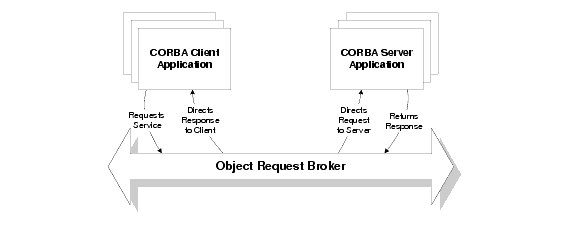
\includegraphics[width=12cm]{corba.png}
\caption{Schéma simplifié de la communication CORBA dans une architecture client-serveur}
\label{ddcanalyse}
\end{center}
\end{figure}

Pour pouvoir utiliser ce serveur, on doit simplement utiliser des objets implémentant les interfaces qu'il fournis. Le principe est le suivant :

\begin{itemize}
\item On récupère les interfaces du serveur, par compilation du fichier idl ou dans un .jar fourni par le serveur 
\item on récupère à partir de l'orb l'objet qui nous intéresse (l'objet Serveur dans le cas présent), à partir de son adresse, de son port et de son noms (également fournis)
\item on invoque directement sur cet objet les méthodes qui nous intéressent, en passant en paramètre (le cas échéant) les objets implémentant les interfaces requises.
\item on récupère le résultat de cet appel de méthode de manière classique
\end{itemize}

L'utilisation de l'objet distant est ainsi complètement transparente, la seule contrainte étant que les objets passés en paramètre ou en retour de méthode doivent être sérializables.

\chapter{Travail réalisé}

\minitoc

\section{De l'intérêt de l'analyse...}

Avant de commencer cette partie, il est important de rappeler que nos choix concernant la manière de communiquer devait respecter les contraintes du serveur. Nous avons donc décidé, après concertation entre les différentes équipes "clientes" et l'équipe "serveur", que le serveur choisirait de son coté la manière de communiquer, et que les clients devraient ensuite respecter ces interfaces. C'était probablement la solution la plus simple et la plus efficace, car essayer de mettre d'accord en même temps différents groupes ayant chacun réalisé une analyse différente aurait pris autant de temps que le projet lui-même. Cependant, l'absence d'un chef global de projet, ou de toute personne ayant une vue globale de tous les travaux, associée à la consigne de ne pas mettre ces travaux en commun avant la conception détaillée nous a réservé de mauvaises surprises.

En effet, une fois les interfaces du serveur prêtes, il s'est avéré que certains éléments de notre modèle étaient incompatibles avec le modèle que mettait à notre disposition le serveur. Nous reviendrons sur ces dysfonctionnement et sur ce qui aurait pu être fait pour l'éviter dans la partie "discussion".
	
Néanmoins, nous avons pu contourner en partie les incompatibilités entre les interfaces du serveur et notre modèle, en utilisant le pattern "décorateur". Pour chaque classe ne pouvant être utilisée tel quel, nous avons créé une classe implémentant l'interface serveur désirée, et contenant l'objet issu de la classe de notre modèle. Toutes les méthodes de l'interface sont implémentées pour utiliser cet objet, ou pour "simuler" la présence de certains éléments le cas échéant. Nous pouvions ainsi fournir au serveur des objets implémentant ses interfaces, sans pour autant modifier de fond en comble notre modèle.

\section{Fonctionnement du serveur}

L'équipe de création du serveur a anticipé un problème pouvant survenir : les appels de méthodes, en Corba (comme ailleurs), se font de manière synchrone. Estimant(à juste titre) que cela pourrais poser des problèmes, leur choix s'est porté sur une manière inhabituelle d'utiliser ce système : le callback.
	
L'utilisation de ce "pattern" permet de simuler l'asynchrone à partir d'un système fonctionnant normalement de manière synchrone. Le concept est simple : en paramètre de chaque méthode, le client devra passer en plus des autres arguments un objet implémentant l'interface "callback", paramétré par le type de retour attendu de la méthode, mais dont l'implémentation est laissée au client. Ainsi, au lieu d'utiliser le "return" des méthodes, le serveur appelle la méthode "onSuccess" présente dans l'interface callback, mais qui sera appelée sur l'objet distant se trouvant sur notre machine.
	
Bien qu'elle implique une charge supplémentaire de travail (implémentation des "callback" correspondant à chaque type de requête), cette façon de faire est plutôt ingénieuse. Nous n'avons cependant pas eu le loisir de la tester, comme nous allons l'expliquer dans la partie Critique et Discussion.

Le Serveur dispose également d'un système de compte : la première fois qu'un utilisateur désire se connecter, il doit créer un nouveau compte, ou s'identifier avec un compte existant, en envoyant le login et le mot de passe correspondant. Le serveur renvoie alors un jeton d'identification, qui sera envoyé avec toutes les autres requêtes, et qui permettra d'identifier l'appelant.
	
\section{Utilisation du serveur}

Afin d'utiliser ce serveur, nous avons implémenté un ensemble de classes dans le package "communicationServeur", permettant une utilisation simple des fonctionnalités du serveur à partir du coeur de l'application. L'objet "façade" de ce package instancie la classe "ProxyServeur", dont les méthodes principales sont les suivantes : 
	
\begin{itemize}
\item connect() : permet de récupérer l'instance de l'objet CORBA Serveur, comme décrit dans [approche théorique - Description],puis appelle la méthode "login(..)" sur cette instance. C'est cette instance qui sera utilisée pour l'appel des autres méthodes. La méthode "onSuccess" du CallBack passé en paramètre de "login(..)" permet à la fois de récupérer le jeton d'identification, et de fixer le booleen "estConnecte" du proxyServeur à vrai.

\item disconnect() : appel de la méthode "disconnect()" sur l'objet serveur, et destruction de cette instance (on devra à nouveau appeler la méthode "connect" pour communiquer avec le serveur)

\item actualiserClient()  : méthode permettant de récupérer sur le serveur les éléments du compte, en appelant successivement sur l'instance du serveur les méthodes " downloadContexte", "downloadIdees", "downloadTache", "downloadProjet". A chacune de ces méthodes est associé un callBack particulier, permettant de récupérer une liste des éléments demandés. On fait ensuite appel à la classe Merger pour fusionner les éléments du serveur avec ceux présents sur la machine. Le fait d'utiliser une classe de fusion séparée permet d'avoir plusieurs méthodes de mise à jour(écrasement systématique, demande à l'utilisateur systématique, ou plus subtil...).
Il est à noter que l'on peut très aisément concevoir d'ajouter un paramètre à la méthode actualiserClient, afin par exemple de ne récupérer qu'un sous-ensemble des taches et projets contenus dans ce compte.

\item actualiserServeur() :  méthode divisée en deux parties : envoi des "ChosesAFaire" au serveur (pour toutes les choses à faire de la liste, on invoque la méthode "créerIdee" du serveur), et envoi de tout le contenu d'un projet (le projet racine si on désire tout envoyer) au serveur. L'envoi de tous les projets s'effectue à l'aide d'un visiteur, visitant tous les éléments du projet, et appliquant un traitement différent selon qu'il rencontre un projet ordonné, un projet non ordonné ou une tache. Dans le cas de la tache, on vérifiera d'abord que toutes les entités(contexte, contacts,...) qui y sont contenues sont bien présentes sur le serveur. Pour cela, on dispose de deux HashMap contenues dans TransformeurDeTache, qui permettent de faire le lien entre les identifiants serveur et les identifiants locaux de chaque entité. Dans le cas ou l'identifiant local n'est pas contenu dans ces tables, l'objet n'existe pas sur le serveur et on utilise donc la méthode "créer<Element>", dont le callback renvoie l'identifiant serveur de l'objet créé, qu'on ajoute alors dans les tables.

\end{itemize}

\chapter{Critique et discussion}

\minitoc

Dans cette partie nous reviendrons sur les éléments critiquables de la solution proposée, et essaierons de proposer un modèle alternatif pour une telle architecture.

Il convient tout d'abord d'expliquer en quoi l'application n'a pas pu marcher. Le problème est très simple : le langage idl ne permet pas d'utiliser des types génériques. Le principe du callback reposant sur sa généricité, il n'était pas possible de l'utiliser sans cet aspect. Il y avait donc un conflit entre le type du callback généré par la compilation du fichier idl, qui était celui que nous devions utiliser dans les appels de méthodes du serveur, et le type générique qui nous avait été fourni précédemment, à partir duquel nous avions implémenté nos propres CallBack.

Voyons maintenant en quoi nous aurions pu éviter cette situation.

\section{Gestion du projet}
Un élément très simple et pourtant primordial est la façon dont le projet a été géré dans sa globalité. En fait il n'y a pas eu de gestion de projet à proprement parler, chaque groupe s'est occupé de sa partie, en se tenant au courant des avancement et des contraintes des autres groupes de manière informelle et décousue. A un stade assez avancé (trop avancé) de la conception, il nous est apparu, aux autres groupes et à nous, que l'équipe du serveur aurait du avoir de l'avance sur nous, et qu'en réalité nous aurions utiliser leurs interfaces déjà prêtes pour concevoir notre modèle. Cela nous aurait permis d'éviter notre incompatibilité de modèles, et de constater plus tôt les problèmes engendrés par l'utilisation du callback, et d'y apporter des solutions, comme par exemple des convertisseur permettant de créer des callbacks non-templaté à partir de callbacks génériques. Cette solution aurait bien sur été assez difficile dans notre cadre, car toutes les équipes commencent au même moment, et disposent du même temps.

Une autre solution aurait été de mettre nos travaux en commun après la phase d'analyse. Nous aurions pu ainsi soit dégager un modèle en prenant un peu de chacun, soit choisir l'un des modèles, que tout le monde utiliserait par la suite. Cela aurait également permis d'éviter l'incompatibilité de modèles.


\section{Alternative}

Alternativement, on peut envisager le cas classique, sans utilisation du callback. Les différences principales auraient été que nous aurions récupéré directement les résultats des appels de méthodes distants, et nous aurions donc du effectuer le traitement directement à la suite. On aurait donc eu un code plus dense, où les requêtes au serveur ne seraient pas séparées du code métier suivant ces requêtes. L'autre différence importante est que nous aurions alors du placer exécuter les appels aux méthodes du serveur dans un thread, car ces appels distants peuvent prendre un certain temps, et seraient bloquants pour l'application si on ne les mettais pas dans un thread séparé.



\chapter*{Conclusion}

L'élaboration de ce projet nous a permis de mieux cerner les différentes problématiques liées à l'utilisation d'une architecture CORBA, et nous a également permis de confronter les notions vues en cours avec un cas concret. Cela nous a par exemple montré les conséquences que peut avoir le choix d'un certain modèle, et l'importance de spécifier auparavant les interfaces qui permettront la communication. Nous avons également pu avoir une réflexion sur les modes de communication synchrone ou asynchrone, et tenter d'utiliser une solution pour simuler l'asynchrone à partir du synchrone. Toutefois nous avons pu constater les problèmes technique sue cela posait, et il est probable qu'à l'avenir nous éviteront ce type de solution si elle n'est pas réellement nécessaire.

\end{document}
